% ================================================================
\chapter{Complexidade de algoritmos}\label{cap:complex}\label{sec:complex}
% ================================================================
\begin{objetivos}
\begin{itemize}
  \item Medir o custo de um algoritmo em função do tamanho da entrada: pior caso, caso médio e melhor caso.
  \item As notações assintóticas $O$, $\Omega$, $\Theta$, $o$ e $\omega$ e suas propriedades.
  \item Analisar laços na prática: como contar as iterações de um trecho de código.
  \item A diferença entre a complexidade de um \emph{algoritmo} e a de um \emph{problema}: limites superiores, inferiores e algoritmos ótimos.
  \item Por que a fronteira entre algoritmos polinomiais e exponenciais importa, e o que é um algoritmo pseudopolinomial.
\end{itemize}
\end{objetivos}

Dois programas que resolvem o mesmo problema podem levar tempos muito diferentes. Considere a tarefa de calcular a soma $1+2+\cdots+N$. Um programa faz um laço que soma os números um a um; outro usa a fórmula de Gauss, $N(N+1)/2$.
\begin{figura}
\begin{minipage}[t]{0.42\linewidth}
\begin{pseudo}{Soma com laço}
\begin{algorithmic}
\State $s:=0$
\For{$i:=1$ \textbf{até} $N$} \State $s:=s+i$ \EndFor
\State \Return $s$
\end{algorithmic}
\end{pseudo}
\end{minipage}\hspace{0.06\linewidth}%
\begin{minipage}[t]{0.42\linewidth}
\begin{pseudo}{Soma com a fórmula}
\begin{algorithmic}
\State \Return $N(N+1)/2$
\end{algorithmic}
\end{pseudo}
\end{minipage}
\end{figura}
Para $N=10$, ambos são instantâneos. Para $N=10^{12}$, o primeiro faz um trilhão de somas e o segundo continua fazendo três operações. A diferença não está na máquina nem na linguagem: está no \emph{número de passos} que cada algoritmo executa e em \emph{como esse número cresce} quando a entrada aumenta.

Este capítulo fixa a linguagem que será usada no resto do livro para fazer esse tipo de comparação. As técnicas para resolver recorrências aparecem no Capítulo~\ref{cap:sortcomp}, junto com o primeiro algoritmo recursivo estudado, e a análise amortizada aparece no Capítulo~\ref{cap:heapav}.

\section{Medidas de complexidade}\label{sec:medidas}
\begin{intuicao}
Medir um algoritmo pelo tempo de relógio é pouco confiável: o mesmo programa roda em tempos diferentes em computadores diferentes. Em vez disso, contamos \textbf{passos elementares} (uma comparação, uma soma, uma atribuição, um acesso a uma posição de vetor), cada um com custo constante, e expressamos o total como uma \emph{função do tamanho da entrada}.
\end{intuicao}

O problema é que entradas do mesmo tamanho podem dar trabalhos diferentes. Fixe um algoritmo $A$ e um tamanho de entrada $n$. Sejam $E_1,\dots,E_m$ todas as entradas possíveis de tamanho $n$ e $T_i$ o número de passos que $A$ executa sobre $E_i$. Há três maneiras naturais de resumir os números $T_1,\dots,T_m$ num só valor:
\begin{itemize}
  \item a complexidade de \textbf{pior caso}, $\max_iT_i$;
  \item a complexidade de \textbf{caso médio}, $\sum_ip_iT_i$, onde $p_i$ é a probabilidade de a entrada ser $E_i$;
  \item a complexidade de \textbf{melhor caso}, $\min_iT_i$.
\end{itemize}

\begin{exemplo}[Os três casos da ordenação por inserção]\label{ex:inscasos}
A ordenação por inserção percorre o vetor da esquerda para a direita e insere cada elemento na posição correta entre os anteriores, que já estão ordenados. Para isso, compara o elemento com os anteriores, do mais próximo para o mais distante, até achar um menor ou chegar ao início.
\begin{figura}[Ordenação por inserção sobre $[3,1,4,2]$. Em cada linha, o elemento destacado é inserido entre os anteriores (já ordenados); à direita, as comparações feitas.]
\begin{tikzpicture}[x=7mm,y=8mm]
\foreach \lin/\vals/\h/\cmt in {0/{3,1,4,2}/2/{1 comparação},1/{1,3,4,2}/3/{1 comparação},2/{1,3,4,2}/4/{3 comparações},3/{1,2,3,4}/0/{}}{
  \foreach \x [count=\i] in \vals {
    \ifnum\i=\h \fill[destaque] (\i-0.5,-\lin-0.35) rectangle (\i+0.5,-\lin+0.35); \fi
    \node[cel] at (\i,-\lin) {\x};}
  \node[rot,anchor=west] at (5,-\lin) {\cmt};}
\node[rot,anchor=east] at (0.3,0) {$j=2$};
\node[rot,anchor=east] at (0.3,-1) {$j=3$};
\node[rot,anchor=east] at (0.3,-2) {$j=4$};
\node[rot,anchor=east] at (0.3,-3) {fim};
\end{tikzpicture}
\end{figura}
Para $n=4$, as 24 ordens possíveis de quatro números distintos dão:
\begin{itemize}
  \item \textbf{melhor caso}: o vetor já ordenado, $[1,2,3,4]$; cada elemento é comparado só com o vizinho e não se move: $3$ comparações, e em geral $n-1$;
  \item \textbf{pior caso}: o vetor decrescente, $[4,3,2,1]$; cada elemento é comparado com todos os anteriores: $1+2+3=6$ comparações, e em geral $n(n-1)/2$;
  \item \textbf{caso médio}, supondo as 24 ordens igualmente prováveis: a média é $59/12\approx4{,}92$ comparações (a entrada $[3,1,4,2]$ da figura faz 5).
\end{itemize}
O mesmo algoritmo é linear em entradas favoráveis e quadrático nas desfavoráveis.
\end{exemplo}

O pior caso é a medida padrão: ele dá uma \emph{garantia} que vale para toda entrada, e não depende de hipóteses sobre a distribuição das entradas, que nem sempre são realistas. O caso médio é útil quando essa distribuição é conhecida (o quicksort, por exemplo, é rápido em média e lento no pior caso). O melhor caso raramente diz algo útil, mas aparece para mostrar que um algoritmo pode ser rápido em entradas favoráveis, como a ordenação por inserção num vetor já ordenado.

Uma quarta medida, a complexidade \textbf{amortizada}, divide o custo de uma \emph{sequência} de operações sobre uma estrutura de dados pelo número de operações, no pior caso da sequência. Ela não envolve probabilidade e será estudada no Capítulo~\ref{cap:heapav}.

\subsection*{Tamanho da entrada}
O tamanho de uma entrada é o comprimento da sua codificação, em bits ou em símbolos. Para uma lista de $n$ números de tamanho limitado, o tamanho é proporcional a $n$. Mas quando a entrada é um número $N$, ela ocupa apenas cerca de $\log_2 N$ bits (ou $\log_{10}N$ dígitos), e um algoritmo cujo custo cresce com o \emph{valor} de $N$ pode ser exponencial no tamanho da entrada.

\begin{exemplo}[A soma com laço é exponencial no número de dígitos]\label{ex:somalaco}
Volte à soma $1+2+\cdots+N$. O laço faz $N$ iterações, o que parece ``linear''. Mas a entrada é o próprio número $N$, escrito com $d\approx\log_{10}N$ dígitos:
\begin{center}\small
\begin{tabular}{@{}rrr@{}}
\toprule
dígitos de $N$ & iterações do laço & tempo a $10^9$ iterações/s\\
\midrule
$3$ & $10^3$ & $1$ microssegundo\\
$9$ & $10^9$ & $1$ segundo\\
$15$ & $10^{15}$ & $\approx 11{,}6$ dias\\
$30$ & $10^{30}$ & $\approx3\cdot10^{13}$ anos\\
\bottomrule
\end{tabular}
\end{center}
Cada dígito a mais multiplica o tempo por 10: o custo é $\Theta(10^d)$, exponencial no tamanho $d$ da entrada. A fórmula $N(N+1)/2$, por outro lado, faz uma multiplicação de números com $d$ dígitos, o que custa $O(d^2)$ pelo método escolar: polinomial.
\end{exemplo}

Um algoritmo é \textbf{pseudopolinomial} quando é polinomial no \emph{valor} dos números da entrada (isto é, quando eles são escritos em unário), mas não necessariamente no seu tamanho em bits. A soma com laço é um exemplo artificial; exemplos importantes são o \emph{counting sort} do Capítulo~\ref{cap:sortlin}, de custo $\Theta(n+k)$ para inteiros em $[0,k]$, e a programação dinâmica para a mochila do Capítulo~\ref{cap:pd}, de custo $\Theta(nW)$.

\section{Notações assintóticas}\label{sec:notacoes}
\begin{intuicao}
Quando $n$ é grande, só o termo que cresce mais rápido importa. Em $n^2+10n+20$, para $n=1000$ o termo $n^2$ vale $10^6$, enquanto $10n+20$ vale $10\,020$, cerca de $1\%$ do total. E constantes multiplicativas dependem da máquina: um computador duas vezes mais rápido transforma $2n^2$ em $n^2$. Por isso dizemos simplesmente que esse custo ``é da ordem de $n^2$''. As notações assintóticas tornam essa frase precisa.
\end{intuicao}

As notações abaixo valem para funções $f,g$ não negativas a partir de algum ponto. Leia $f=O(g)$ como ``$f$ cresce no máximo como $g$''.
\begin{center}
\begin{tabular}{@{}llll@{}}
\toprule
Notação & Definição & Via limite (se existir) & Leitura\\
\midrule
$f=O(g)$ & $\exists c>0,n_0:\ f(n)\le c\,g(n)\ \forall n\ge n_0$ & $\lim f/g<\infty$ & ``$\le$''\\
$f=\Omega(g)$ & $\exists c>0,n_0:\ f(n)\ge c\,g(n)\ \forall n\ge n_0$ & $\lim f/g>0$ & ``$\ge$''\\
$f=\Theta(g)$ & $f=O(g)$ e $f=\Omega(g)$ & $\lim f/g=c\in(0,\infty)$ & ``$=$''\\
$f=o(g)$ & $\forall c>0\ \exists n_0:\ f(n)<c\,g(n)\ \forall n\ge n_0$ & $\lim f/g=0$ & ``$<$''\\
$f=\omega(g)$ & $\forall c>0\ \exists n_0:\ f(n)>c\,g(n)\ \forall n\ge n_0$ & $\lim f/g=\infty$ & ``$>$''\\
\bottomrule
\end{tabular}
\end{center}
Formalmente, $O(g)$ é um \emph{conjunto} de funções, e $f=O(g)$ significa $f\in O(g)$; o sinal de igualdade é um abuso de notação consagrado, que deve ser lido sempre da esquerda para a direita ($n=O(n^2)$ está certo; ``$O(n^2)=n$'' não faz sentido).

\subsection*{As notações $O$, $\Omega$ e $\Theta$ numa figura}
A definição de $O$ tem duas constantes, e cada uma tem um papel: $c$ absorve as constantes multiplicativas, e $n_0$ permite ignorar os valores pequenos de $n$, onde termos de ordem menor ainda pesam. A Figura~\ref{fig:otheta} mostra as duas em ação.

\begin{figura}[A função $f(n)=n^2+10n+20$ fica ``ensanduichada'' entre $1\cdot n^2$ e $2\cdot n^2$ a partir de $n_0=12$. A curva de baixo prova $f=\Omega(n^2)$, a de cima prova $f=O(n^2)$ e as duas juntas provam $f=\Theta(n^2)$.\label{fig:otheta}]
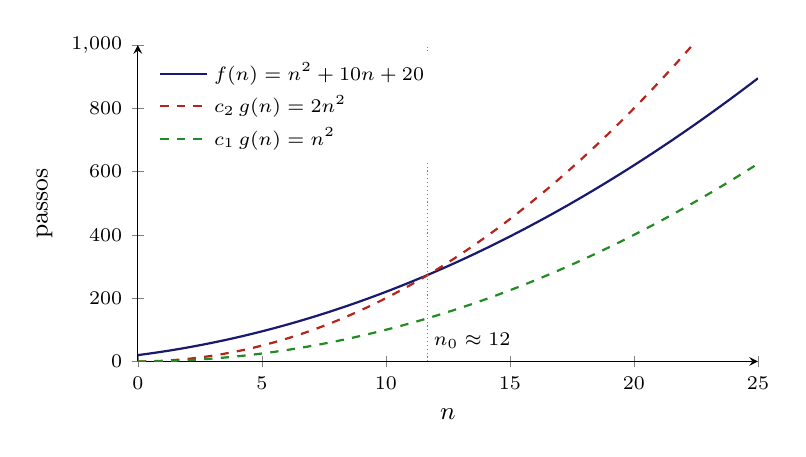
\begin{tikzpicture}
\begin{axis}[width=0.78\linewidth, height=5.6cm, domain=0:25, samples=60, xmin=0, xmax=25, ymin=0, ymax=1000,
  axis lines=left, xlabel={$n$}, ylabel={passos}, ylabel style={font=\small}, xlabel style={font=\small},
  tick label style={font=\scriptsize}, legend style={font=\scriptsize, draw=none, at={(0.02,0.98)}, anchor=north west},
  legend cell align=left]
\addplot[thick, MidnightBlue] {x^2+10*x+20}; \addlegendentry{$f(n)=n^2+10n+20$}
\addplot[thick, BrickRed, dashed] {2*x^2}; \addlegendentry{$c_2\,g(n)=2n^2$}
\addplot[thick, ForestGreen, dashed] {x^2}; \addlegendentry{$c_1\,g(n)=n^2$}
\draw[gray, densely dotted] (axis cs:11.66,0) -- (axis cs:11.66,1000);
\node[font=\scriptsize, anchor=south west, fill=white, inner sep=1pt] at (axis cs:11.8,30) {$n_0\approx 12$};
\end{axis}
\end{tikzpicture}
\end{figura}

\begin{exemplo}[Provando $O$, $\Omega$ e $\Theta$ pela definição]\label{ex:otheta}
Seja $f(n)=n^2+10n+20$.
\begin{itemize}
  \item $f=O(n^2)$: queremos $c$ e $n_0$ com $n^2+10n+20\le c\,n^2$. Com $c=2$, a desigualdade vira $10n+20\le n^2$, que vale para $n\ge12$ (para $n=12$: $140\le144$). Logo $c=2$, $n_0=12$ servem. Também serviria $c=31$, $n_0=1$, pois $10n\le10n^2$ e $20\le20n^2$ para $n\ge1$: as constantes não são únicas, basta exibir \emph{uma} escolha.
  \item $f=\Omega(n^2)$: com $c=1$ e $n_0=1$, $f(n)\ge n^2$ é óbvio.
  \item $f=\Theta(n^2)$: segue dos dois itens. Note que $f$ também é $O(n^3)$ (um limite superior folgado), mas \emph{não} é $O(n)$: se fosse, existiria $c$ com $n^2\le f(n)\le c\,n$ para $n$ grande, ou seja, $n\le c$, o que é falso para $n>c$.
\end{itemize}
\end{exemplo}

\begin{exemplo}
Pela mesma técnica, a função $4n^3+5n$ é $O(n^4)$ e $O(n^3)$, mas não é $O(n^2)$; é $\Omega(n^2)$ e $\Omega(n^3)$, mas não é $\Omega(n^4)$; portanto é $\Theta(n^3)$. Para provar $4n^3+5n=O(n^3)$ pela definição, basta tomar $c=9$ e $n_0=1$: $4n^3+5n\le4n^3+5n^3=9n^3$ para todo $n\ge1$.
\end{exemplo}

\subsection*{As versões estritas $o$ e $\omega$}
Em $f=O(g)$, a função $f$ pode crescer \emph{tanto quanto} $g$; em $f=o(g)$, ela cresce \emph{estritamente menos}: para \emph{qualquer} constante $c$, por menor que seja, $f$ acaba ficando abaixo de $c\,g$. A diferença está no quantificador: em $O$ basta \emph{existir} um $c$, em $o$ a desigualdade vale \emph{para todo} $c$.

\begin{exemplo}[Usando limites]\label{ex:limites}
Quando o limite de $f/g$ existe, ele resolve tudo de uma vez:
\begin{itemize}
  \item $\displaystyle\lim_{n\to\infty}\frac{3n^2+5n}{n^2}=3$, um número em $(0,\infty)$: logo $3n^2+5n=\Theta(n^2)$.
  \item $\displaystyle\lim\frac{n}{n^2}=\lim\frac1n=0$: logo $n=o(n^2)$. Já $n^2\ne o(n^2)$, pois $n^2/n^2=1\not\to0$.
  \item $\displaystyle\lim\frac{\ln n}{\sqrt n}=\lim\frac{1/n}{1/(2\sqrt n)}=\lim\frac{2}{\sqrt n}=0$ (regra de L'Hôpital): logo $\log n=o(\sqrt n)$. Logaritmos crescem mais devagar que qualquer raiz.
  \item $\displaystyle\lim\frac{2^n}{n^3}=\infty$ (aplique L'Hôpital três vezes): logo $2^n=\omega(n^3)$. Exponenciais crescem mais rápido que qualquer polinômio.
\end{itemize}
\end{exemplo}

\subsection*{Propriedades}
As notações se comportam como as desigualdades que representam:
\begin{itemize}
  \item \textbf{transitividade}: $f=O(g)$ e $g=O(h)$ implicam $f=O(h)$ (e o mesmo para as outras notações);
  \item \textbf{simetria transposta}: $f=O(g)$ se e somente se $g=\Omega(f)$;
  \item \textbf{a soma é dominada pela maior parcela}: $f+g=\Theta(\max\{f,g\})$;
  \item \textbf{a base do logaritmo não importa}: $\log_an=\log_bn/\log_ba$ difere de $\log_bn$ pelo fator constante $1/\log_ba$.
\end{itemize}

\begin{exemplo}[Aplicando as propriedades]\label{ex:propriedades}\leavevmode
\begin{itemize}
  \item $5n^3+100\,n^2\log n+7=\Theta(n^3)$: a soma é dominada pela maior parcela, e $n^2\log n=o(n^3)$ porque $\log n=o(n)$.
  \item $\log_{10}n=\log_2n/\log_2 10\approx0{,}301\log_2n$; logo $\log_{10}n=\Theta(\log_2n)$, e podemos escrever simplesmente $\Theta(\log n)$.
  \item $\log(n^3)=3\log n=\Theta(\log n)$, mas $\log(3^n)=n\log3=\Theta(n)$: o expoente \emph{dentro} do logaritmo vira constante; o expoente que depende de $n$, não.
\end{itemize}
\end{exemplo}

Também valem $\log(n!)=\Theta(n\log n)$, $(\log n)^c=o(n^\varepsilon)$ para quaisquer $c>0$ e $\varepsilon>0$, e $n^c=o(a^n)$ para todo $a>1$. A escala abaixo resume as ordens de crescimento mais frequentes:
\[
1\ <\ \log\log n\ <\ \log n\ <\ \sqrt n\ <\ n\ <\ n\log n\ <\ n^2\ <\ n^3\ <\ n^{\log n}\ <\ 2^n\ <\ n!\ <\ n^n .
\]

\begin{figura}[As funções mais comuns para $n$ entre 1 e 20. Para $n$ pequeno, todas parecem próximas; logo a exponencial $2^n$ sai do gráfico, e $n^2$ se afasta de $n\log n$.\label{fig:crescimento}]
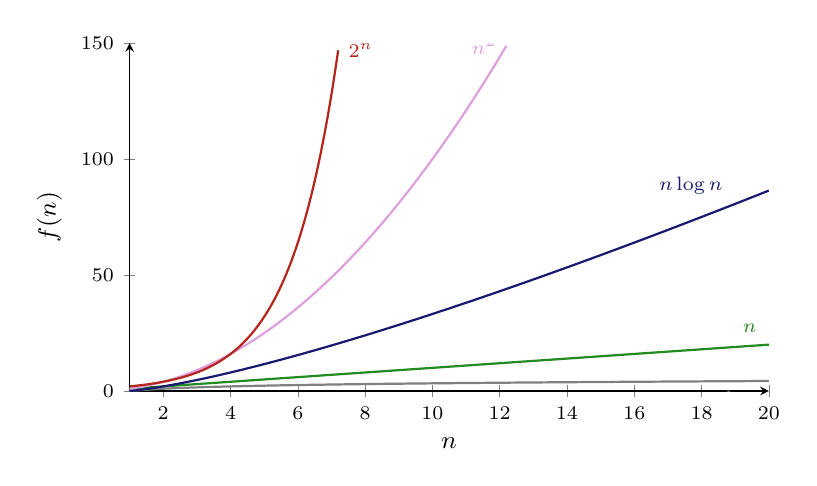
\begin{tikzpicture}
\begin{axis}[width=0.8\linewidth, height=6cm, domain=1:20, samples=80, xmin=1, xmax=20, ymin=0, ymax=150,
  axis lines=left, xlabel={$n$}, ylabel={$f(n)$}, tick label style={font=\scriptsize},
  xlabel style={font=\small}, ylabel style={font=\small}, clip=true,
  every axis plot/.append style={thick}]
\addplot[gray] {log2(x)} node[pos=0.97, below, font=\scriptsize] {$\log n$};
\addplot[ForestGreen] {x} node[pos=0.97, above=1pt, font=\scriptsize] {$n$};
\addplot[MidnightBlue] {x*log2(x)} node[pos=0.93, above left, font=\scriptsize] {$n\log n$};
\addplot[Plum, domain=1:12.2] {x^2} node[pos=1, left, font=\scriptsize] {$n^2$};
\addplot[BrickRed, domain=1:7.2] {2^x} node[pos=1, right, font=\scriptsize] {$2^n$};
\end{axis}
\end{tikzpicture}
\end{figura}

A Tabela~\ref{tab:tempos} traduz essas ordens em tempo real, supondo um computador que executa um bilhão de passos por segundo. Ela mostra por que a ordem de crescimento importa mais que qualquer constante.
\begin{figura}
\captionof{table}{Tempo para executar $f(n)$ passos a $10^9$ passos por segundo.}\label{tab:tempos}
\small
\begin{tabular}{@{}rcccccc@{}}
\toprule
$n$ & $\log n$ & $n$ & $n\log n$ & $n^2$ & $n^3$ & $2^n$\\
\midrule
$10$ & 3\,ns & 10\,ns & 33\,ns & 100\,ns & 1\,$\mu$s & 1\,$\mu$s\\
$100$ & 7\,ns & 100\,ns & 664\,ns & 10\,$\mu$s & 1\,ms & $4\cdot10^{13}$ anos\\
$1000$ & 10\,ns & 1\,$\mu$s & 10\,$\mu$s & 1\,ms & 1\,s & ---\\
$10^6$ & 20\,ns & 1\,ms & 20\,ms & 17\,min & 32 anos & ---\\
\bottomrule
\end{tabular}
\end{figura}

\section{Analisando laços na prática}\label{sec:lacos}
Na maior parte das vezes, analisar um algoritmo iterativo é contar quantas vezes o corpo dos seus laços é executado.

\begin{roteiro}[Como analisar um trecho com laços]
\begin{enumerate}
  \item Identifique o \textbf{corpo mais interno} e verifique que ele custa $O(1)$.
  \item Para cada laço, escreva quantas vezes ele itera \emph{em função das variáveis dos laços externos}.
  \item Some: laços aninhados viram somatórios aninhados.
  \item Resolva o somatório e simplifique com as notações assintóticas.
\end{enumerate}
\end{roteiro}

\begin{exemplo}[Três padrões de laço]\label{ex:lacos}
\textbf{(a) Laços aninhados independentes.} Em ``\textbf{para} $i:=1$ \textbf{até} $n$, \textbf{para} $j:=1$ \textbf{até} $n$: corpo'', o corpo executa $n\cdot n=n^2$ vezes: $\Theta(n^2)$.

\smallskip
\textbf{(b) Laço interno que depende do externo.} Em ``\textbf{para} $i:=1$ \textbf{até} $n$, \textbf{para} $j:=1$ \textbf{até} $i$: corpo'', o laço interno faz $i$ iterações, e o total é
\[
\sum_{i=1}^n i=\frac{n(n+1)}2=\Theta(n^2).
\]
A Figura~\ref{fig:escada} mostra a contagem como uma escada: as execuções ocupam cerca de metade do quadrado $n\times n$, e metade de $n^2$ ainda é $\Theta(n^2)$.

\smallskip
\textbf{(c) Laço que divide pela metade.} Em ``$i:=n$; \textbf{enquanto} $i>1$ \textbf{faça} $i:=\floor{i/2}$'', o valor de $i$ passa por $n,\ n/2,\ n/4,\dots$ até chegar a $1$. Depois de $k$ iterações, $i\approx n/2^k$, que chega a $1$ quando $k\approx\log_2n$: $\Theta(\log n)$. Para $n=16$, $i$ vale $16,8,4,2,1$: quatro iterações.
\end{exemplo}

\begin{figura}[O laço do item (b) com $n=6$: na linha $i$, o corpo executa $i$ vezes (células preenchidas). O total, $1+2+\cdots+6=21$, é pouco mais que a metade das 36 células.\label{fig:escada}]
\begin{tikzpicture}[x=6mm,y=6mm]
\foreach \i in {1,...,6}{
  \foreach \j in {1,...,6}{
    \ifnum\j>\i \draw[gray!40] (\j-1,-\i) rectangle (\j,-\i+1);
    \else \draw[fill=azul] (\j-1,-\i) rectangle (\j,-\i+1); \fi}
  \node[rot,anchor=east] at (-0.2,-\i+0.5) {$i=\i$};
  \node[rot,anchor=west] at (6.2,-\i+0.5) {\i\ execuções};}
\node[rot] at (3,0.5) {$j=1,\dots,6$};
\end{tikzpicture}
\end{figura}

Um laço cuja variável é multiplicada ou dividida por uma constante a cada passo dá $\Theta(\log n)$ iterações. É isso que torna a \textbf{busca binária} tão rápida: a cada comparação, o trecho do vetor ordenado onde o elemento procurado pode estar cai pela metade.

\begin{figura}[Busca binária de $x=27$ num vetor ordenado de 16 posições. O trecho candidato (em destaque) cai pela metade a cada comparação com o elemento do meio ($\blacktriangledown$).\label{fig:buscabin}]
\begin{tikzpicture}[x=6.4mm,y=7.5mm]
\foreach \lin/\a/\b/\m in {0/1/16/8,1/9/16/12,2/9/11/10,3/11/11/11}{
  \fill[destaque] (\a-0.5,-\lin-0.32) rectangle (\b+0.5,-\lin+0.32);
  \foreach \x [count=\i] in {2,5,8,12,15,16,19,21,23,25,27,30,34,40,41,47}{
    \node[cel, minimum width=6.4mm, font=\scriptsize] at (\i,-\lin) {\x};}
  \node[font=\tiny] at (\m,-\lin+0.5) {$\blacktriangledown$};}
\node[rot,anchor=west] at (16.8,0) {$27>21$: direita};
\node[rot,anchor=west] at (16.8,-1) {$27<30$: esquerda};
\node[rot,anchor=west] at (16.8,-2) {$27>25$: direita};
\node[rot,anchor=west] at (16.8,-3) {achou!};
\end{tikzpicture}
\end{figura}

\begin{cuidado}[Erros comuns na análise de laços]
\begin{itemize}
  \item Multiplicar os limites dos laços quando o interno depende do externo: isso sempre dá um limite \emph{superior}, mas ele pode ser folgado. No item (b) a ordem saiu certa; no Exercício~\ref{ex:cx-lacos}(a), em que $i$ dobra a cada volta, faça a soma com cuidado antes de concluir.
  \item Esquecer que $\Theta$ descarta constantes: $n(n+1)/2$ e $n^2$ são da mesma ordem.
  \item Confundir o número de iterações com o \emph{valor} das variáveis: em (c), $i$ começa em $n$, mas o laço só dá $\log_2 n$ voltas.
\end{itemize}
\end{cuidado}

\section{Complexidade de problemas e de algoritmos}\label{sec:problemas}
A complexidade de um \emph{algoritmo} é uma função que descreve o seu custo. A complexidade de um \emph{problema} é uma pergunta mais difícil: qual o menor custo possível entre \emph{todos} os algoritmos que o resolvem, inclusive os que ainda não foram inventados?

\begin{defi}\leavevmode
\begin{itemize}
  \item Uma função $f(n)$ é um \textbf{limite superior} para o problema $\Pi$ se \emph{existe} algum algoritmo que resolve $\Pi$ com no máximo $f(n)$ passos no pior caso. A complexidade de pior caso de qualquer algoritmo para $\Pi$ é um limite superior para $\Pi$.
  \item Uma função $f(n)$ é um \textbf{limite inferior} para $\Pi$ se \emph{todo} algoritmo que resolve $\Pi$ executa pelo menos $f(n)$ passos no pior caso.
  \item Um algoritmo é \textbf{ótimo} se sua complexidade de pior caso coincide com um limite inferior do problema.
\end{itemize}
\end{defi}

\begin{exemplo}[Encontrar o máximo é um problema de custo exatamente $n-1$]\label{ex:maximo}
Considere o problema de achar o maior de $n$ números distintos usando comparações.
\begin{itemize}
  \item \textbf{Limite superior}: o algoritmo que guarda o maior visto até agora e o compara com cada novo elemento faz $n-1$ comparações. Logo $n-1$ é um limite superior para o problema.
  \item \textbf{Limite inferior}: numa comparação ``$a<b$?'', diremos que o menor dos dois \emph{perdeu}. Um algoritmo só pode ter certeza de que $x$ é o máximo se cada um dos outros $n-1$ elementos já perdeu alguma comparação: se $y\ne x$ nunca perdeu, $y$ poderia ser o máximo sem contradizer nenhuma resposta obtida. Como cada comparação produz exatamente um perdedor, são necessárias pelo menos $n-1$ comparações, \emph{qualquer que seja o algoritmo}.
\end{itemize}
Os dois limites coincidem, e o algoritmo simples é ótimo.
\begin{figura}[O máximo de $[5,9,2,7]$. Cada comparação (seta) elimina um candidato, o perdedor (em vermelho). Com $n=4$ elementos, três perdedores exigem três comparações.]
\begin{tikzpicture}[x=1.6cm]
\node[vtx] (a) at (0,0) {5}; \node[vtx] (b) at (1,0) {9}; \node[vtx] (c) at (2,0) {2}; \node[vtx] (d) at (3,0) {7};
\node[vtx, fill=ruim] (a1) at (0.5,-1.1) {5}; \node[vtx] (b1) at (1.5,-1.1) {9};
\node[vtx, fill=ruim] (c2) at (2,-2.2) {2}; \node[vtx] (b2) at (1,-2.2) {9};
\node[vtx, fill=ruim] (d3) at (3,-3.3) {7}; \node[vtx, fill=feito] (b3) at (1.5,-3.3) {9};
\node[rot, anchor=west] at (3.3,-1.1) {$5<9$: 5 perde};
\node[rot, anchor=west] at (3.3,-2.2) {$2<9$: 2 perde};
\node[rot, anchor=west] at (3.3,-3.3) {$7<9$: 7 perde};
\draw[seta,gray] (a) -- (a1); \draw[seta,gray] (b) -- (b1);
\draw[seta,gray] (b1) -- (b2); \draw[seta,gray] (c) -- (c2);
\draw[seta,gray] (b2) -- (b3); \draw[seta,gray] (d) -- (d3);
\end{tikzpicture}
\end{figura}
\end{exemplo}

Limites superiores se provam exibindo um algoritmo; limites inferiores exigem um argumento sobre todos os algoritmos possíveis, como o argumento do exemplo acima ou o da árvore de decisão, que mostra que ordenar por comparações exige $\Omega(n\log n)$ comparações (Capítulo~\ref{cap:sortcomp}). O mergesort e o heapsort, que fazem $O(n\log n)$ comparações, são portanto ótimos.

As notações assintóticas são afirmações sobre funções, e não sobre ``limites'' no sentido acima: nada impede dizer que o pior caso de um algoritmo é $\Omega(n^3)$, ou que conhecemos para um problema um limite inferior que é $O(\log n)$.

\section{Algoritmos polinomiais e exponenciais}\label{sec:polinomiais}
Um algoritmo é \textbf{polinomial} se seu custo de pior caso é $O(n^c)$ para alguma constante $c$; a classe dos problemas que admitem algoritmos polinomiais é chamada de $P$. Custos como $2^n$, $k^n$, $n!$, $2^{n^2}$ e $n^{\log n}$ são \textbf{exponenciais} (ou superpolinomiais).

O consenso é que algoritmos polinomiais são eficientes e exponenciais não, por um motivo que vai além do tempo absoluto da Tabela~\ref{tab:tempos}: algoritmos polinomiais aproveitam o avanço tecnológico. Com uma máquina mais rápida, o maior tamanho de entrada resolvido num tempo fixo é \emph{multiplicado} por uma constante quando o custo é polinomial, mas apenas \emph{acrescido} de uma constante quando é exponencial.

\begin{exemplo}[O que uma máquina 100 vezes mais rápida compra]\label{ex:maquina}
Suponha que hoje, em uma hora, resolvemos entradas de tamanho até $N$. Com a máquina nova, no mesmo tempo, fazemos $100$ vezes mais passos:
\begin{center}\small
\begin{tabular}{@{}lll@{}}
\toprule
custo & novo tamanho máximo & por quê\\
\midrule
$n$ & $100N$ & $n'=100N$ dá $100N$ passos\\
$n^2$ & $\sqrt{100}\,N=10\,N$ & $(10N)^2=100N^2$\\
$n^3$ & $\sqrt[3]{100}\,N\approx4{,}64\,N$ & $(4{,}64N)^3\approx100N^3$\\
$2^n$ & $N+6{,}6$ & $2^{N+6{,}6}\approx100\cdot2^N$\\
\bottomrule
\end{tabular}
\end{center}
Se hoje resolvemos $N=1000$ com o algoritmo quadrático, passaremos a resolver $10\,000$. Se resolvemos $N=40$ com o exponencial, passaremos a resolver só $46$: cem vezes mais velocidade compram seis posições a mais.
\end{exemplo}

\begin{chave}
Pior caso é a medida padrão. $O$ é ``$\le$'', $\Omega$ é ``$\ge$'', $\Theta$ é ``$=$'' a menos de constantes, para $n$ grande; a base do logaritmo não importa. Laços aninhados viram somatórios; laços que dividem a variável por uma constante dão $\Theta(\log n)$ voltas. Limite superior de um problema: \emph{existe} um algoritmo; limite inferior: \emph{todo} algoritmo; ótimo: pior caso igual ao limite inferior. O tamanho da entrada se mede em bits, e algoritmos cujo custo cresce com o \emph{valor} de um número são pseudopolinomiais.
\end{chave}

% ----------------------------------------------------------------
\section{Exercícios}
\excurso
\begin{exercicio}{cx-slide}[Slides]<ex:otheta>
Diga, justificando pela definição, se $2n^2+1$ é: (a) $O(n)$; (b) $O(n^2)$; (c) $O(n^3)$; (d) $\Omega(n)$; (e) $\Omega(n^3)$; (f) $\Theta(n^2)$.
\end{exercicio}
\begin{exercicio}{cx-tec}[Slides]<ex:maquina>
Uma máquina nova é 10 vezes mais rápida que a antiga. Para algoritmos de custo $n$, $n^2$ e $2^n$, em quanto aumenta o maior tamanho de entrada que se resolve no mesmo tempo? O que isso diz sobre algoritmos polinomiais e exponenciais?
\end{exercicio}
\begin{exercicio}{cx-k}[Slides]<sec:medidas>
O \emph{counting sort} ordena $n$ inteiros em $[0,k]$ em tempo $\Theta(n+k)$. Explique por que ele \textbf{não} é polinomial no tamanho da entrada quando $k=2^n$, e por que é linear quando $k=O(n)$.
\end{exercicio}

\excompl
\begin{exercicio}{cx-ordem}[Complementar]<sec:notacoes>
Ordene as funções pela taxa de crescimento: $\sqrt n$,\ $\log^2 n$,\ $2^{\log_2 n}$,\ $n\log n$,\ $n^{\log_2 3}$,\ $1{,}01^n$,\ $n^{100}$,\ $n!$,\ $2^{2^n}$.
\end{exercicio}
\begin{exercicio}{cx-vf}[Complementar]<ex:propriedades>
Verdadeiro ou falso? Justifique.
(a) $2^{n+1}=O(2^n)$;\quad (b) $2^{2n}=O(2^n)$;\quad (c) $\log(n^2)=\Theta(\log n)$;\quad (d) $(\log n)^{100}=O(n^{0{,}01})$;\quad (e) $n^{\log n}=O(2^n)$;\quad (f) se $f=O(g)$ então $2^{f}=O(2^{g})$.
\end{exercicio}
\begin{exercicio}{cx-fat}[Complementar]<sec:notacoes>
Mostre que $\log(n!)=\Theta(n\log n)$ sem usar a fórmula de Stirling.
\end{exercicio}
\begin{exercicio}{cx-incomp}[Complementar]<sec:notacoes>
Dê funções positivas $f$ e $g$ tais que nem $f=O(g)$ nem $g=O(f)$.
\end{exercicio}
\begin{exercicio}{cx-lacos}[Complementar]<ex:lacos>
Dê a complexidade, em $\Theta$, de cada trecho (o corpo mais interno custa $O(1)$):
\begin{center}\small
\begin{minipage}{0.45\linewidth}
(a)\ $i:=1$\\
\textbf{enquanto} $i\le n$ \textbf{faça}\\
\hspace*{1em}\textbf{para} $j:=1$ \textbf{até} $i$ \textbf{faça} (corpo)\\
\hspace*{1em}$i:=2i$
\end{minipage}
\begin{minipage}{0.45\linewidth}
(b)\ \textbf{para} $i:=1$ \textbf{até} $n$ \textbf{faça}\\
\hspace*{1em}$j:=1$\\
\hspace*{1em}\textbf{enquanto} $j\le n$ \textbf{faça}\\
\hspace*{2em}(corpo);\ $j:=2j$
\end{minipage}
\end{center}
\end{exercicio}
\begin{exercicio}{cx-primo}[Complementar]<ex:somalaco>
O algoritmo que testa se $N$ é primo tentando dividir $N$ por $2,3,\dots,\floor{\sqrt N}$ faz $O(\sqrt N)$ divisões. Ele é polinomial? (Pense no tamanho da entrada.)
\end{exercicio}
\begin{exercicio}{cx-def3}[Complementar]<ex:otheta>
Prove pela definição, exibindo as constantes, que $3n^3-100n^2+7=\Theta(n^3)$.
\end{exercicio}
\begin{exercicio}{cx-nlogn}[Complementar]<ex:otheta>
Prove que $n^2\ne O(n\log n)$.
\end{exercicio}
\begin{exercicio}{cx-base}[Complementar]<ex:propriedades>
Prove que, para quaisquer constantes $a,b>1$, $\log_an=\Theta(\log_bn)$. Por que, por outro lado, $a^n$ e $b^n$ não são da mesma ordem quando $a\ne b$?
\end{exercicio}
\begin{exercicio}{cx-prop}[Complementar]<sec:notacoes>
Prove: (a) se $f=O(g)$ e $g=O(h)$, então $f=O(h)$; (b) $f+g=\Theta(\max\{f,g\})$; (c) $f=\Theta(g)$ se e somente se $g=\Theta(f)$.
\end{exercicio}
\begin{exercicio}{cx-somak}[Complementar]<ex:lacos>
Mostre que $\sum_{i=1}^ni^k=\Theta(n^{k+1})$ para toda constante inteira $k\ge1$.
\end{exercicio}
\begin{exercicio}{cx-harm}[Complementar]<sec:notacoes>
Mostre que $H_n=\sum_{i=1}^n\frac1i=\Theta(\log n)$, comparando a soma com a integral de $1/x$.
\end{exercicio}
\begin{exercicio}{cx-busca}[Complementar]<sec:medidas>
Na busca sequencial de $x$ num vetor de $n$ elementos distintos, quantas comparações são feitas no pior caso, no melhor caso e no caso médio, supondo que $x$ está no vetor e é igualmente provável em cada posição?
\end{exercicio}
\begin{exercicio}{cx-triplo}[Complementar]<ex:lacos>
Quantas vezes o corpo é executado no trecho ``\textbf{para} $i:=1$ \textbf{até} $n$, \textbf{para} $j:=i$ \textbf{até} $n$, \textbf{para} $k:=i$ \textbf{até} $j$: corpo''? Dê a fórmula exata e a ordem em $\Theta$.
\end{exercicio}
\begin{exercicio}{cx-loglog}[Complementar]<ex:lacos>
Qual a complexidade do trecho ``$j:=2$; \textbf{enquanto} $j\le n$ \textbf{faça} $j:=j^2$''?
\end{exercicio}
\begin{exercicio}{cx-fatexp}[Complementar]<ex:limites>
Mostre que $2^n=o(n!)$ e que $n!=o(n^n)$.
\end{exercicio}
\begin{exercicio}{cx-binaria}[Complementar]<fig:buscabin>
Quantas comparações a busca binária faz no pior caso num vetor ordenado com 1000 elementos? E com $10^6$? Dê a fórmula geral.
\end{exercicio}
\begin{exercicio}{cx-inf}[Complementar]<ex:maximo>
Mostre que todo algoritmo que decide se $x$ está num vetor \emph{não ordenado} de $n$ elementos, usando apenas comparações de $x$ com elementos do vetor, faz pelo menos $n$ comparações no pior caso. Conclua que a busca sequencial é ótima nesse modelo.
\end{exercicio}
\begin{exercicio}{cx-max}[Complementar]<ex:propriedades>
Verdadeiro ou falso? (a) $\max\{f,g\}=\Theta(f+g)$; (b) $f=O(g)$ implica $\log f=O(\log g)$, para $f,g\ge2$; (c) $f=O(g)$ implica $f^2=O(g^2)$; (d) $f(n)=O(f(n/2))$ para toda $f$ crescente.
\end{exercicio}
\begin{exercicio}{cx-insercao4}[Complementar]<ex:inscasos>
Conte as comparações que a ordenação por inserção do Exemplo~\ref{ex:inscasos} faz nas entradas $[2,4,1,3]$ e $[4,3,1,2]$, inserção por inserção. Por que a segunda faz tantas comparações quanto o vetor decrescente $[4,3,2,1]$, embora não seja decrescente?
\end{exercicio}
\begin{exercicio}{cx-tercos}[Complementar]<ex:lacos>
Quantas vezes o laço ``$i:=n$; \textbf{enquanto} $i>1$ \textbf{faça} $i:=\floor{i/3}$'' é executado para $n=100$ e para $n=1000$? Dê uma fórmula para $n\ge2$ e a ordem em $\Theta$.
\end{exercicio}
